\documentclass{article}
\usepackage{amsmath}
\usepackage[mathletters]{ucs}
\usepackage[utf8x]{inputenc}
\usepackage[margin=1.5in]{geometry}
\usepackage{enumerate}
\newtheorem{theorem}{Theorem}
\usepackage[dvipsnames]{xcolor}
\usepackage{pgfplots}
\setlength{\parindent}{0cm}
\usepackage{graphics}
\usepackage{graphicx} % Required for including images
\usepackage{subcaption}
\usepackage{bigintcalc}
\usepackage{pythonhighlight} %for pythonkode \begin{python}   \end{python}
\usepackage{appendix}
\usepackage{arydshln}
\usepackage{physics}
\usepackage{tikz-cd}
\usepackage{booktabs} 
\usepackage{adjustbox}
\usepackage{mdframed}
\usepackage{relsize}
\usepackage{physics}
\usepackage[thinc]{esdiff}
\usepackage{fixltx2e}
\usepackage{esint}  %for lukket-linje-integral
\usepackage{xfrac} %for sfrac
\usepackage[colorlinks=true]{hyperref} %for linker, må ha med hypersetup
\usepackage[noabbrev, nameinlink]{cleveref} % to be loaded after hyperref
\usepackage{amssymb} %\mathbb{R} for reelle tall, \mathcal{B} for "matte"-font
\usepackage{listings} %for kode/lstlisting
\usepackage{verbatim}
\usepackage{graphicx,wrapfig,lipsum,caption} %for wrapping av bilder
\usepackage{mathtools} %for \abs{x}
\usepackage[norsk]{babel}
\definecolor{codegreen}{rgb}{0,0.6,0}
\definecolor{codegray}{rgb}{0.5,0.5,0.5}
\definecolor{codepurple}{rgb}{0.58,0,0.82}
\definecolor{backcolour}{rgb}{0.95,0.95,0.92}
\lstdefinestyle{mystyle}{
    backgroundcolor=\color{backcolour},   
    commentstyle=\color{codegreen},
    keywordstyle=\color{magenta},
    numberstyle=\tiny\color{codegray},
    stringstyle=\color{codepurple},
    basicstyle=\ttfamily\footnotesize,
    breakatwhitespace=false,         
    breaklines=true,                 
    captionpos=b,                    
    keepspaces=true,                 
    numbers=left,                    
    numbersep=5pt,                  
    showspaces=false,                
    showstringspaces=false,
    showtabs=false,                  
    tabsize=2
}

\lstset{style=mystyle}
\author{Oskar Idland}
\title{Oblig 5}
\date{}
\begin{document}
\maketitle
\newpage
\section*{Problem 1}
\subsection*{a)}
\begin{figure}[h!]
\centering
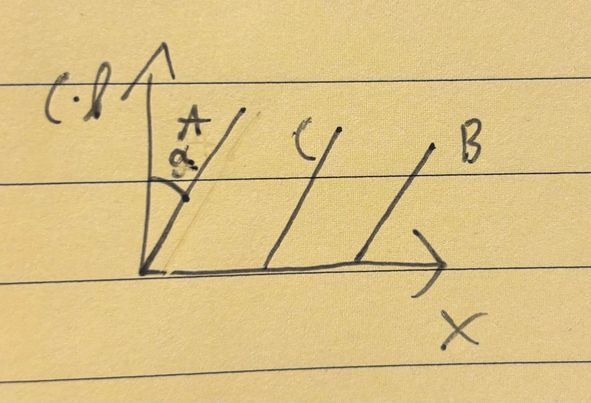
\includegraphics[width = \textwidth]{1a.jpg}
\caption{Minkowski diagram}
\label{fig: 1a}
\end{figure}

The velocity is represented by the angle between the $y$-axis and the world line. We have constant velocity $v$ and can use the fact that the world line passes through the origin. Therefore, the velocity is given by $v = x_{A}(t) / t$. We can represent the slope of the world line as $\tan α = v / c$. 

\subsection*{b)}
\begin{figure}[h!]
\centering
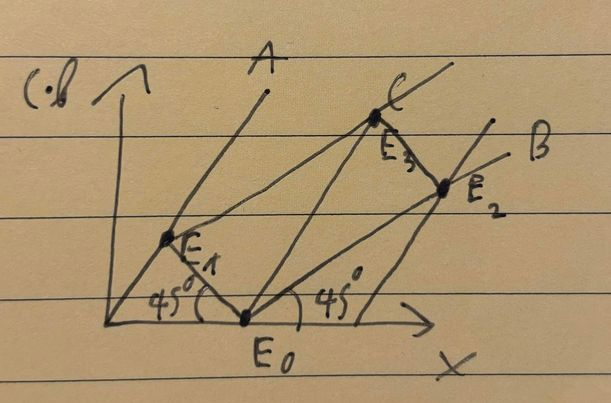
\includegraphics[width = \textwidth]{1b.jpg}
\caption{Minkowski diagram with events} 
\label{fig: 1b}
\end{figure}
As light travels at the speed of light, it will appear as a $45^{∘}$ angle. 


\subsection*{c)}
From the perspective of $S'$, it would seem like none of the points where moving. The light travels an equal distance in event $E_1$ and $E_2$ and will therefore appear simultaneous. The drawing from problem b, is not correct from this POV. 

\subsection*{d)}
See \cref{fig: 1b}. 

\subsection*{e)}


\section*{Problem 2}
\subsection*{a)}
As the rod is moving along the $y$-axis, there will not be any length contraction in the $x$-direction. Point $B$ is located at the end of the rod, with a distance to point $A$ of $L_0 / 2$. This gives us $x_{B}' = L_0 / 2$. Both $y$ coordinates move at velocity $u$. It is only represented by a different time coordinate. We therefore get $y_{B}' = ut'_{B}$. As we neither move in the $z$-direction nor have different values in each point, their coordinates are the same, meaning $z_{B}' = z_{A}' = 0$. 

\subsection*{b)}
Using the Lorentz transformation, we get the following:
\[
x_{A} = γ(x_a' + vt_{A}') = γvt_{A}'
\]
\[
x_{B} = γ(x_b' + vt_{B}') = γ(L_0 / 2 + vt_{B}')
\]
\[
y_{A} = ut_{A}' 
\]
\[
y_{B} = ut_{B}'
\]
\[
z_{A} = z_{B} = 0
\]
\[
t_{A} = γ(t_{A}' + vx_{A}' / c^2) = γt_{A}'
\]
\[
t_{B} = γ(t_{B}' + vx_{B}' / c^2) = γ(t_{B}' + v(L_0 / 2) / c^2)
\]
Now we must convert from the primed to the unprimed system. We can use the following:
\[
t_{A}' = t_{A} / γ 
\]
\[
t_{B}' = t_{B} / γ - vL_0 / (2c^2)
\]
We can now insert these into the equations for $x_{A}$ and $x_{B}$:
\[
x_{A} = γv(t_{A} / γ) = vt_{A}
\]
\[
x_{B} = γ(L_0 / 2 + v(t_{B} / γ - vL_0 / (2c^2))) = γL_0 / 2 + vt_{B} - γv^2L_0 / (2c^2)
\]
And for $y_{A}$ and $y_{B}$:
\[
y_{A} = ut_{A} / γ
\]
\[
y_{B} = ut_{B} / γ - uvL_0 / (2c^2)
\]

\subsection*{c)}
\[
\tan ϕ = \frac{y_{B} - y_{A}}{x_{B} - x_{A}}
\]
We insert the expressions for $x_{A}$, $x_{B}$, $y_{A}$ and $y_{B}$:
\[
\tan ϕ = -γuv / c^2
\]
As long as $v,u ≠ 0$ we get an angle different from $0$, meaning the rod is not parallel to the $x$-axis.

The length of the rod is just the absolute value of the difference between the start $(x_{A}, y_{A})$ and end $(x_{B}, y_{B})$ of the rod. 
\[
L / 2 = \sqrt{(x_{B} - x_{A})^2 + (y_{B} - y_{A})^2}
\]
\[
L = 2\sqrt{(x_{B} - x_{A})^2 + (y_{B} - y_{A})^2}
\]
\[
L = 2\sqrt{L_0^2 / (4γ^2) + u^2v^2L_0^2 / (4c^4γ^2)}
\]
\[
L = L_0 \sqrt{1 / γ^2 + u^2v^2 / c^4}
\]


\end{document}